\documentclass[../main.tex]{subfiles}
\graphicspath{{\subfix{../img/}}}

\begin{document}

\section{Discussion}

\textit{Drosophila} is a well-established animal model for studying sleep due to its striking similarities in sleep regulation with vertebrates \cite{shaferRegulationDrosophilaSleep2021,andreaniCircadianProgrammingEllipsoid2022}. R5 neurons have been reported to play important role in sleep regulation in the fruit flies. Specifically, these neurons are thought to encode the homeostatic sleep drive in these animals \cite{liuSleepDriveEncoded2016}. Similar to mammals,
\gls{swa} has been observed in \textit{Drosophila} brain during sleep and following sleep deprivation, and is believed to be generated at the level of the R5 neurons \cite{raccugliaNetworkSpecificSynchronizationElectrical2019}. Furthermore, these neurons exhibit tonic spiking activity during the daytime, and bursing at night and after sleep deprivation \cite{suarez-grimaltNeuralArchitectureSleep2021,liuSleepDriveEncoded2016}. 

Descpite these observations, the cellular mechanisms underlying R5 neuronal activity remains poorly understood. Gaining insight into these mechanisms is crucial for better understanding of the cellular basis of sleep regulation in \textit{Drosophila}.
In this study, conductance-based computational models were used to investigate the possible mechanisms responsible for several experimental findings related to the R5 activity.

First, electrophysiological studies in R5 neurons of \textit{Drosophila} have reported that their activity switches bfrom tonic firing during the daytime to bursting during sleep and following sleep deprivation \parencite{liuSleepDriveEncoded2016,suarez-grimaltNeuralArchitectureSleep2021}. A study on gene expression in \textit{Drosophila} identified a negative correlation between the expression of a gene encoding a potassium channel known as \gls{eag} and increased sleep drive \cite{doppSinglecellTranscriptomicsReveals2024}. This study demonstrated that variation in the expression of \gls{eag} channel might be biologically plausible mechanism underlying transition of R5 activity from tonic spiking to bursting, by reducing the number of spikes per burst.

Second, an unpublished study by David Owald, Anatoli Ender, and colleagues reported the existance of slow oscillations on the order of few seconts following the blockde of $Na^+$ channels in Drosophila R5 neurons. These slow oscillations were hypothesized to be mediated by T-type $Ca^{2+}$ channels. However, the results of the current study indicate that $Ca^{2+}$ channels alone cannot explain such slow-frequency oscillations due to their relatively fast kinetics. Therefore, other, or additional mechanisms should be present to account for the observed large interspike intervals.

Third, another unpublished study of David Owald, Anatoli Ender and colleagues reported an increase in the resting membrane potential (defined as the minimum recorded membrane potential during bursting) following knockdown of T-type $Ca^{2+}$ channels in Drosophila R5 neurons. Since calcium currents are depolarizing, in the current work the involvement of $Ca^{2+}$-activated $K^+$ currents was hypothesized. Simulations showed that such a channel could indeed negatively modulate the minimal membrane potential with reduced number of the T-type channels.

\vspace*{0.3cm}
\noindent\textbf{Transition between tonic spiking to bursting}



\vspace*{0.3cm}
\noindent\textbf{Slow-freqeucny oscillations following $Na^{+}$ channel blockade}

\vspace*{0.3cm}
\noindent\textbf{Increase in resting membrane potential following T-type channel knockdown}


\vspace*{0.3cm}
\noindent\textbf{R5 neurons: inhibition-induced bursters?}


\vspace*{0.3cm}
\noindent\textbf{Conductance-based computational models}




\color{orange}

\parencite{krummSlowlyOscillatingBrain2021} implemented R5 and helicon cells based
on Izhikevich model of burstin neurons \parencite{izhikevichSimpleModelSpiking2003}.

\parencite{krummSlowlyOscillatingBrain2021} suggested the inhibitory synapses between R5 and
helicon cells to explain this observation.

\color{red}

------------------------------
IMPORTANT!!!:
\begin{itemize}
    \item Citations from Lauras thesis
    \begin{itemize}
        \item In the Down state, Helicon is entrained to R5's compound rhythmicity via excitatory
        coupling. This leads to a relatively short offset (7 ms) between the two signals
        \item For Helicon in the Down state, we find a much larger and negative offset of 
        -77 ms (fig. 2.34a). We assume this is because Helicon now also receives inhibitory inputs
        from R5 neurons which prevent Helicon from firing and therefore lead to a small anti-phase
        correlation between the two signals.
    \end{itemize}
    \item From Manuscript:
    \begin{itemize}
        \item (Simulations). This is also in line with our experimental data, which show
        that the balance controls the degree of synchronization between excitatory and inhibitory
        drive and determines whether the networks are in the shifted or synchronized configuration
    \end{itemize}
    \item Remarks
    \begin{itemize}
        \item In the Lauras thesis, in the second note it should be written "Up State" instead of
        "Down State". However, this state
        corresponds to daytime rather than night. Thus this will not explain the experimental
        observations (shifted state at night)
        \item In manuscript, 1) there is no inhibition from R5 to helicon at night. Thus,
        the temporal shift might be due to the synaptic time constant between helicon and R5,
        rather than interplay between excitation and inhibition between R5 and Helicon.
        Synaptic time constant was set to be 100 ms (similar to resulted time delay between helicon and R5).
        Thus, when additional input was provided to helicon, here helicon might drive R5 and R5 might burst due to intrinsic properties.
    \end{itemize}
\end{itemize}

\color{black}


\noindent\hrulefill

\color{orange}

Facts:
\begin{itemize}
    \item Ca1T-null mutants showed increased sleep \parencite{jeongCaa1TFlyTtype2015}
    \item Ca1T in drosophila are located at presynaptic terminals of R5
    
\end{itemize}

\color{red}

Discussion:
\begin{itemize}
    \item Blocking NMDR - irregular interburst interval, controls - regular.
    Chaos??? (further support for square-wave)
    \parencite{raccugliaNetworkSpecificSynchronizationElectrical2019,izhikevichNEURALEXCITABILITYSPIKING2000}
    
    \item Although h current is associated with the repolarizing current (blcking sometimes reduces it),
    h current is not ncessary to observe this phase (examples of simulations).

    \parencite{jeongCaa1TFlyTtype2015} Flies lacking T-Type channels increase amount of sleep. If bursting in
    R5 requires sleep, than this is on the one hand counterintuitive result. Although, knocking down
    expression of T-Type channels in whole fly might have more complex effects on sleep, as other
    circuits that affect R5 acitivty also will lack the similar channel that might result in this
    observation.

    \parencite{blumAstroglialCalciumSignaling2021}: astrocytes and Toll receptors on R5 neurons.
    Toll might trigger gene expression (??? Need a bit more literature research)

    BRP - Important for regulation of calcium channels (???)

    RMP depolarized following SD (Connection to T-Type channels and increased RMP in knockdown.
    Effect of affector circuits following SD, as Ca gated K channels should have the opposite effect ???)
    \parencite{liuSleepDriveEncoded2016}

    \item R5 neurons exhibit 1Hz tonic firing during day and 1Hz tonic firing during night
    \begin{itemize}
        \item According to Liu et al 2016 bursting occurs only in sleep-deprived files (Liu et al 2016). However,
        Raccuglia et al 2019 reported bursting activity at the evening (ZT8-13). The difference might be because
        Liu et al reported above-mentioned results for ZT0. As R5 is modulated by both cyrcadian and homeostatic
        processes (circadian by clock neurons \parencite{doppSinglecellTranscriptomicsReveals2024})
        - this might explain the difference.
        \item Furthermore, I could not find the original paper stating that R5 neurons
        exhibit 1Hz tonic firing during day (Figures \ref{fig:tmp_single_unit_r5_day_night}, \ref{fig:tmp_frequency_vs_zt})
    \end{itemize}

    \item Raccuglia: frequency of R5 activation and locomotion. Actitation was done by optogenetics. If bursting is
    mediated by hyperpolarization activated current, then it can be that optogeneetically one directly
    activates fast system. Thus, you will need specific frequency of activation to induce similar
    effect (intrinsic bursting 1Hz).

    \item Other mechanisms are likely to be involved during normal, undisturbed sleep \parencite{liuSleepDriveEncoded2016}.
    
    \item Manuscript: "Because R5 activation can also entrain
    dFSB activity during the day (Extended Data Fig. 2a-c), we suspect that this interaction would
    effectively set helicon cells to the downstate (night setting), allowing for entrainment of
    helicon by R5."
    \begin{itemize}
        \item This can also be due to DN1p clock neurons, not through dFSB
        \item While helicon cells can be set to the downstate through DN1p-dFSB circuit,
        the SWA could be achieved through R5-helicon-dFSB circuit, where
        excitatory synapses from helicon drive SWA in dFSB. It will be interesting
        to see the time lag correlation between dFSB-helicon and dFSB-R5 in the SD condition.
        Or even better - granger causality (as correlation does not tell us about causality).
        (Paper for method: 
        Reassessing hierarchical correspondences between brain and deep networks through direct interface
        \url{https://www.science.org/doi/10.1126/sciadv.abm2219})
    \end{itemize}

\end{itemize}

\color{black}


    

%% Not ture :)))
% Notably, out of the identified sleep-pressure-inducing neurons, only the inactivation of R5 neurons had effect on
% rebound sleep,  while inactivation of other neurons had no effect. \textcolor{red}{\textbf{(This can be related to the Raccuglia 2019 - reduced neurotransmitter release
% might affect R5 synchronization. Interesting question: as excitatory drive is important for synchronization,
% what will happen if only inhibitory synapses are blocked? No reduction in rebound sleep?)}}

Oscillations after TTX block - neuron might receive external input from other sources
than synaptic current (e.g. gap junctions to other neurons or astrocytes - add citations)

Although for many bursting neurons H current is necessary (blocking of H current blabla, find literature)
it is not mandatory for \gls{ahp} (image from Izhikevich book and models that have ahp but still
have very nice bursts or ahp).

\begin{itemize}
    \item In conntrast to three-compartment mmodel, single-compartment model could only estimate either I-V relationship, or LTS, but not both,
    with LTS observed in case of increased maximal conductance of T-Type channels. \parencite{destexheDendriticLowthresholdCalcium1998}
\end{itemize}


We assume that the R5 neurons are intrinsic bursters, i.e. they can exhibit bursting activity due to
cell-autonomous conductances, even in case of constant input current.
Thus, when concentrating on simulations of R5 neurons to study either transition between
bursting and tonic spiking or effects of blocking specific ion channels, external input to R5 neuron
is modelled as a constant. Furthermore, for simplicity, single compartment conductance based model was chosen.
Such model 1) does not account for dendritic computations, and 2) assumes uniform distribution of
ion channels. \textcolor{green}{Nonlinear interactions in the multi-compartment model might better explain
the experimental results without need of L-Type $Ca^{2+}$ currents.}

Different models
\begin{itemize}
    \item Ion channels
    \item Same model, different parameter regimes
    \item If not mediated by t-type, they do not include T-Type channels
    \item Different goals: inhibition rebound vs induced bursting
    \item Slow variable for calcium oscillations
    \item Misreported parameters (HM neuron in paper and in one thesis)
\end{itemize}

Neurons differ by expression of ion channels, location of ion channels, concentrations. Thus,
different models incorporate different ion channels and max conductances depending on neuron of interest

Single and three compartment neuron model - Destexhe \parencite{destexheDendriticLowthresholdCalcium1998}.

\begin{itemize}
    \item Turrigiano et al 1995 \& Tang: \url{https://pmc.ncbi.nlm.nih.gov/articles/PMC6578228/pdf/jneuro_15_5_3640.pdf}
    \item Fazli et al 2020, Bertram et al 2000: phantom bursting + no sodium
\end{itemize}

EAG: different types (some has only activation, some does not, some are inactivated more by calcium, some not) - two papers on EAG

Do the simulations with noninstantaneous activation for Wang model - maybe the transition between
spiking and resting will be easier

Maybe try to hand-tune one TTX oscillation and then use optimisation to fit others

It is hard to fit generally, as the ion channel dynamics overlap - e.g. extending time constant
might affect other currents and fitting might be the best method

Did not incorporate calcium in day/night - calcium activates k dependent K channels + effectively modulates calcium channel strength -> Thus the effect might be even better

Thing to fit the neurons (blue thing, find what it was)

Slow oscillations in small parameter region - input current is important, as it only affects the V-nullcline. You change it, you move away - you move away from the slow manifold if the trajectory passes along it.

Fast activation of EAG to terminate burst after first spike - generally not required. It is just thought that the R5 fires tonically. However, it can be that it fires only few (e.g. 2) spikes per burst. The model tells, that it can be possible to reduce the number of spikes to 1. However data analysis should be done to see what is in R5 neurons.

switching from day to night will not depend on type of bursting

Different effects with changing one variable also is observed when two parameters are varied (my plot) :D Now you can imagine what will happen in higher dimensions :D

Slow calcium removal and bursting \url{https://pmc.ncbi.nlm.nih.gov/articles/PMC3650241/pdf/10827_2012_Article_430.pdf}

Slow kinetics via slow calcium removal: A Simple biophysically plausible model for long time constants in single neurons.

\begin{figure}[!t]
    \centering
    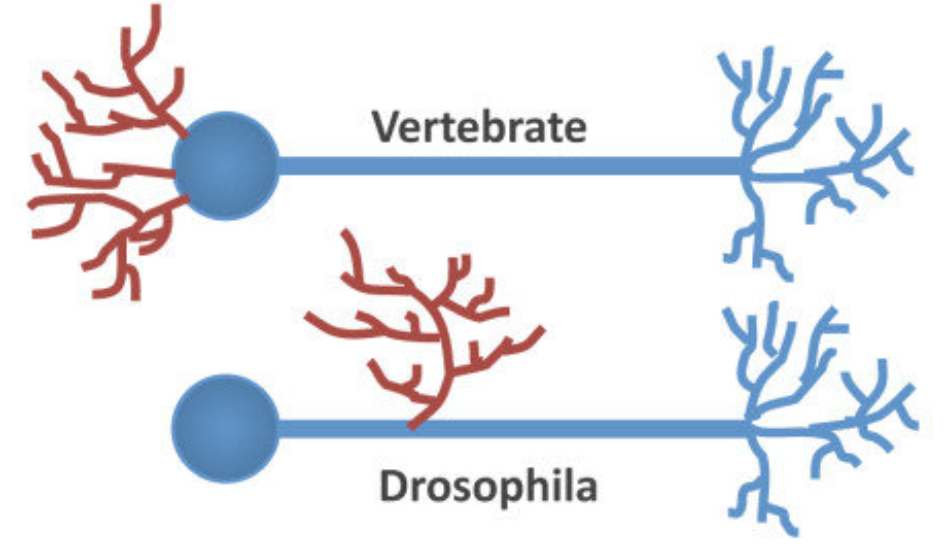
\includegraphics[width=0.55\linewidth]{../img/modeling_r5/examples/drosophila_neuron_morphology.png}
    \caption[Neuron morphology in \textit{Drosophila} and Vertebrates]{
        \textbf{Comparison of neuron morphology in \textit{Drosophila} and Vertebrates.}
        In comparison to vertebrates,
        the neurons in \textit{Drosophila} have unipolar morphology. Therefore synaptic potentials
        travelling from the dendrites (red) to spike initiation zone bypass cell body
        (blue circle). Figure adapted from \parencite{spindlerBazookaMediatesSecondary2011}.
    }
    \label{fig:morphology_drosphila_vs_mammalian}
\end{figure}

Although R5 neurons share similar functional characteristits with thalamic neurons,
morphology of neurons in \textit{Drosophila} is significantly different from those in vertebrates
\ref{fig:morphology_drosphila_vs_mammalian}. 
Unlike vertebrates, \textit{Drosophila} neurons have unipolar morphology. Because of this morphology,
synaptic potentials travelling from dendrites to spike initiation zone bypass cell body.
Because of this morphology, the cell body of \textit{Drosophila} neurons is
electronically segregated from other cell regions, suggesting that it is not involved
in synaptic integration \parencite{gouwensSignalPropagationDrosophila2009,tuthillLessonsCompartmentalModel2009}.
Furthermore, it has been found that, in contrast to vertebrates, dendrites of
\textit{Drosophila} neurons (slecifically, \gls{kc}) are not solely postsynaptic, but
also form presynaptic active zones \parencite{christiansenPresynapsesKenyonCell2011}.


% \item The sharp transient at the end of the pulse in recordings (Fig. \ref{fig:i_v_relationship_jeong})
% is most likely due to passive membrane properties. The membrane time constant of R5 neuons is not known.
% Arbitrarily incorporating $\tau=10$ms time constant reproduced the sharp transient (not shown here).
% However 1) as Drosophila T-Type channels were expressed in frogs (Oocites), fitting membrane time constant
% will not be helpful in modeling Drosophila R5 neurons; 2) The passive membrane time constant

\begin{itemize}
    \item Estimated number of activation gates for Drosophila T-Type ion channels is 3.
    \item modeling the ion channel using Ohmic relationship between current and voltage
    did not procude good fits to observed current-voltage (I-V) relationship.
    \item The current-voltage relationship was reproduced when
    Goldman-Hodgkin-Katz (GHK) voltage flux equation was used instead of Ohmic current
    \item GHK equation models explicit relationship between current, voltage, temperature and
    intra-/extracellular ion concentrations.
    \item The fit of simulated I-V relatoinship to the observed data was improved when
    the steady-state activation function was shifted along $V$ axis,
    and corresponding time constant was scaled and shifted along $V$ axis (parameters for
    shifting and scaling were taken to be free parameters during optimization)
\end{itemize}

\end{document}